\documentclass{article}
\usepackage{amsmath}
\usepackage{graphicx}
\graphicspath{{images/}}
\title{List 1 report}
\author{Albert Kołodziejski}
\begin{document}
\maketitle
\section*{Exercise 1}
\subsection*{Results:}
\begin{center}
    \begin{tabular}{| c | c |}
        \hline
        & MST weight\\ 
        \hline
        XQF131 & 474\\
        \hline
        XQG237 & 897\\
        \hline
        PMA343 & 1179\\
        \hline
        PKA379 & 1151\\
        \hline
        BCL380 & 1444\\
        \hline
        PBL395 & 1124\\
        \hline
        PBK411 & 1180\\
        \hline
        PBN423 & 1201\\
        \hline
        PBM436 & 1269\\
        \hline
        XQL662 & 2240\\
        \hline
    \end{tabular}
    \end{center}
\subsection*{QA:}
\begin{center}
    \textbf{Why weight of MST must be smaller than optimal cycle of salesman?}
\end{center}
If it wasn't smaller, you could take that cycle, remove any edge and in result you will get MST that is smaller, contradiction.

\section*{Exercise 2}
\subsection*{Results:}
\begin{center}
    \begin{tabular}{| c | c |}
        \hline
        & MST Cycle weight\\ 
        \hline
        XQF131 & 758\\
        \hline
        XQG237 & 1456\\
        \hline
        PMA343 & 1861\\
        \hline
        PKA379 & 1838\\
        \hline
        BCL380 & 2341\\
        \hline
        PBL395 & 1819\\
        \hline
        PBK411 & 1870\\
        \hline
        PBN423 & 1944\\
        \hline
        PBM436 & 2053\\
        \hline
        XQL662 & 3650\\
        \hline
    \end{tabular}
    \end{center}
\subsection*{QA:}
\begin{center}
    \textbf{Why weight of cycle made out of MST shouldn't be bigger than weight of tree times 2?}
\end{center}
After visiting all vertexes in some branch in MST.
\begin{center}
    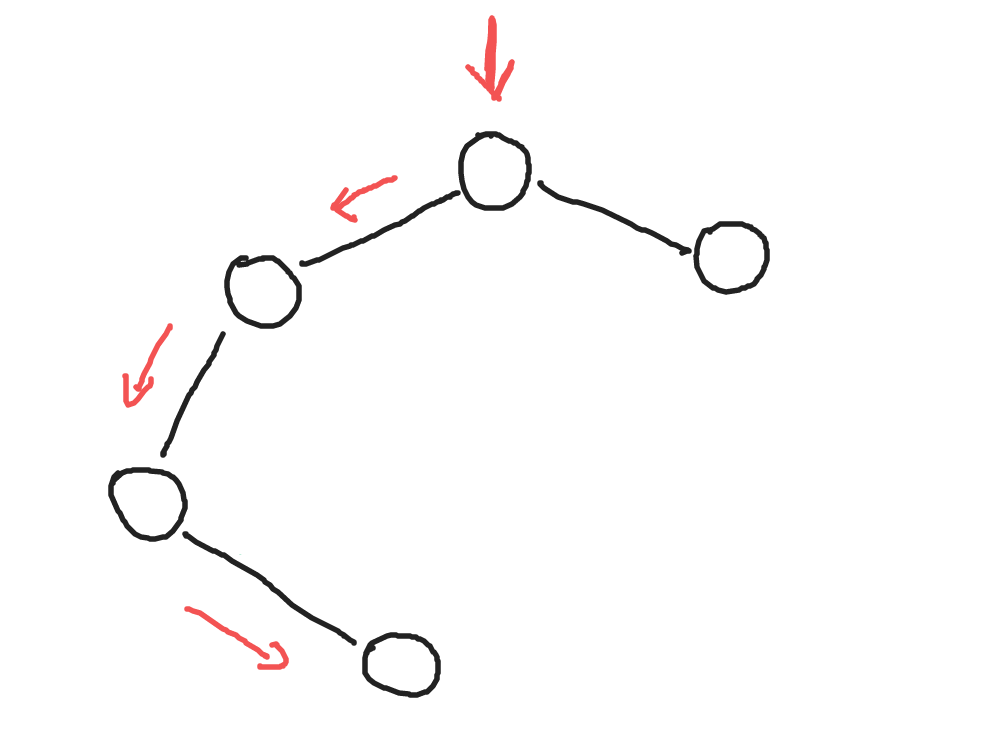
\includegraphics[scale=0.14]{1} 
\end{center}
We will find ourself in situation where we need to use edge outside of MST.
\begin{center}
    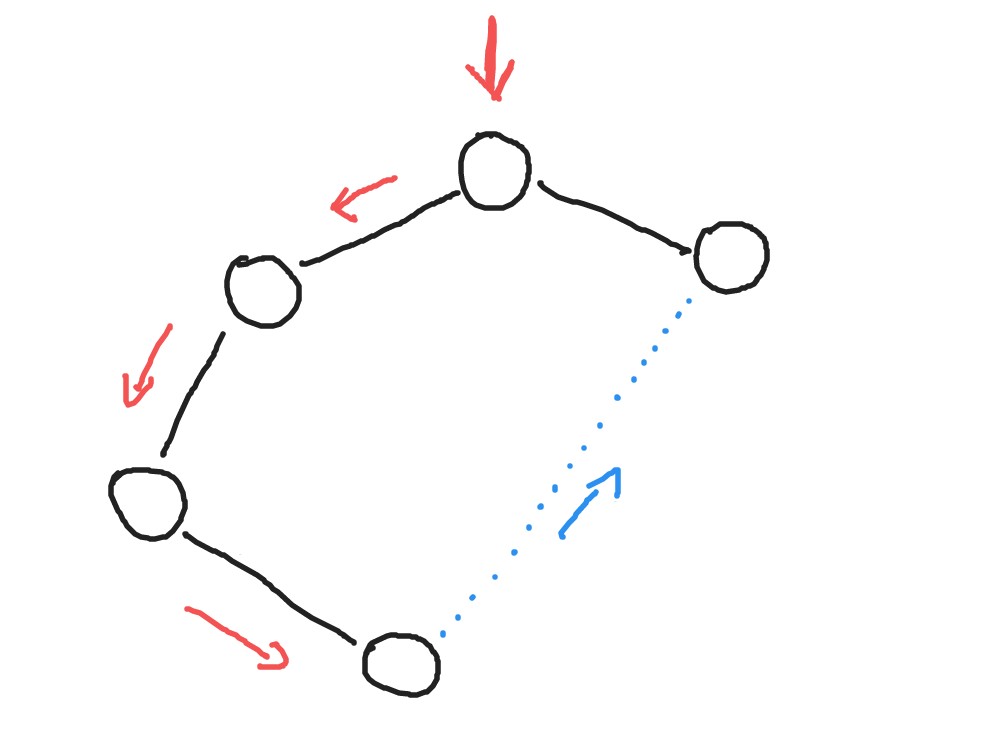
\includegraphics[scale=0.14]{2} 
\end{center}
But because cost function satisfies triangle inequality, we know that direct edge won't have bigger weight than path with aditional vertexes.
\begin{center}
    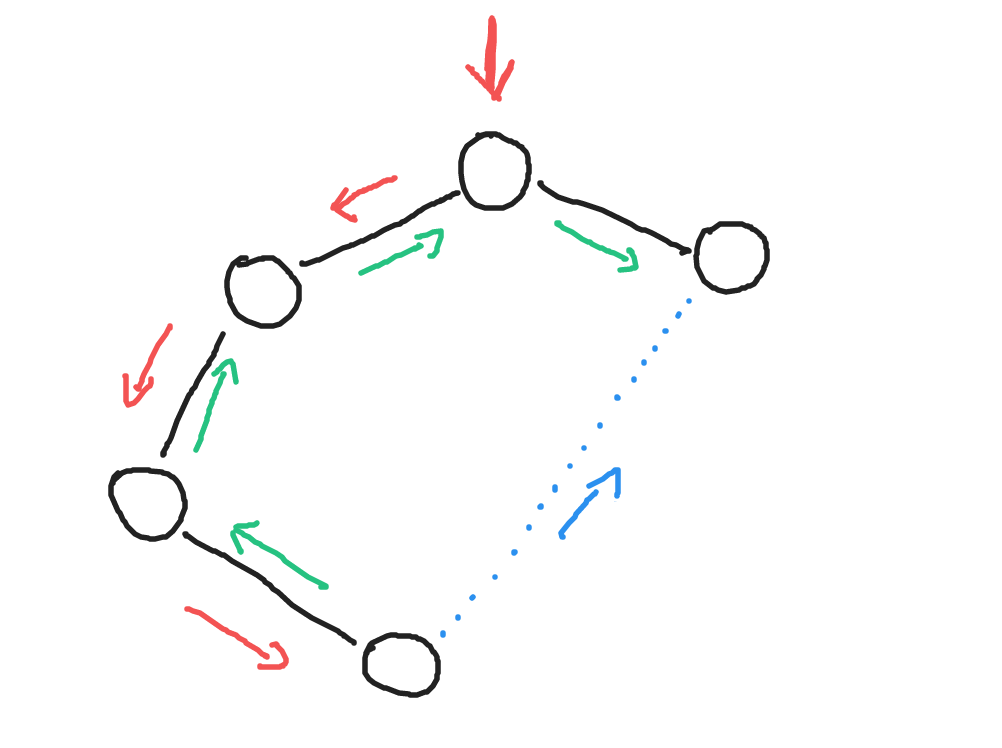
\includegraphics[scale=0.14]{3} 
\end{center}
So blue edge isn't bigger than sum of green edges. Weight in worst case can only double.

\section*{Exercise 3}
\subsection*{Results:}
\begin{center}
    \begin{tabular}{| c | c | c | c |}
        \hline
        & avg from minimal in 10 & afg from minimal in 50 & minimal\\ 
        \hline
        XQF131 & 4337.13 & 4191.15 & 3930\\
        \hline
        XQG237 & 11904.44 & 11628.15 & 11250\\
        \hline
        PMA343 & 34371.73 & 33562.55 & 32485\\
        \hline
        PKA379 & 35393.47 & 34713.3 & 34009\\
        \hline
        BCL380 & 24739.64 & 24334 & 23942\\
        \hline
        PBL395 & 19178.66 & 18909.1 & 18580\\
        \hline
        PBK411 & 21627.48 & 21242.3 & 20497\\
        \hline
        PBN423 & 21935.77 & 21613 & 21296\\
        \hline
        PBM436 & 22469.14 & 22051.65 & 21528\\
        \hline
        XQL662 & 51143.69 & 50552.2 & 49802\\
        \hline
    \end{tabular}
    \end{center}
\subsection*{QA:}
\begin{center}
    \textbf{Does edges can cross in optimal salesman cycle?}
\end{center}
Assume that there is optimal salesman cycle that have edges that cross each other. Let's draw this crossroad that there is a  path in cycle between top two without any bottoms vertexes and vice versa.
\begin{center}
    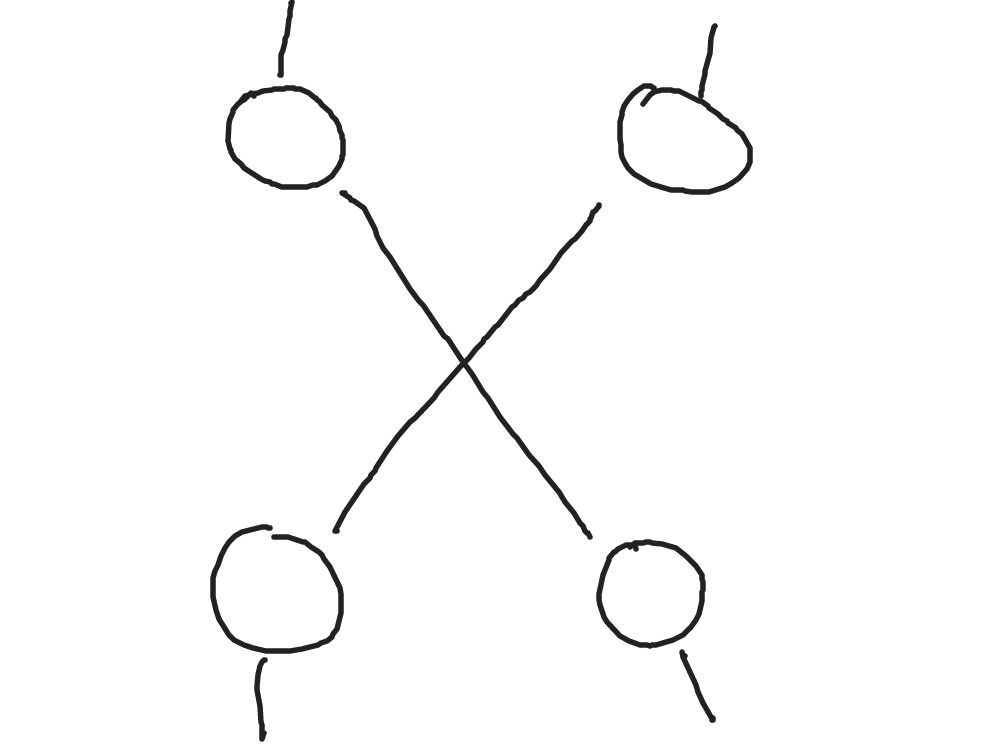
\includegraphics[scale=0.14]{4} 
\end{center}
We can make virtual vertex on crossing, it will split edges into two parts.
\begin{center}
    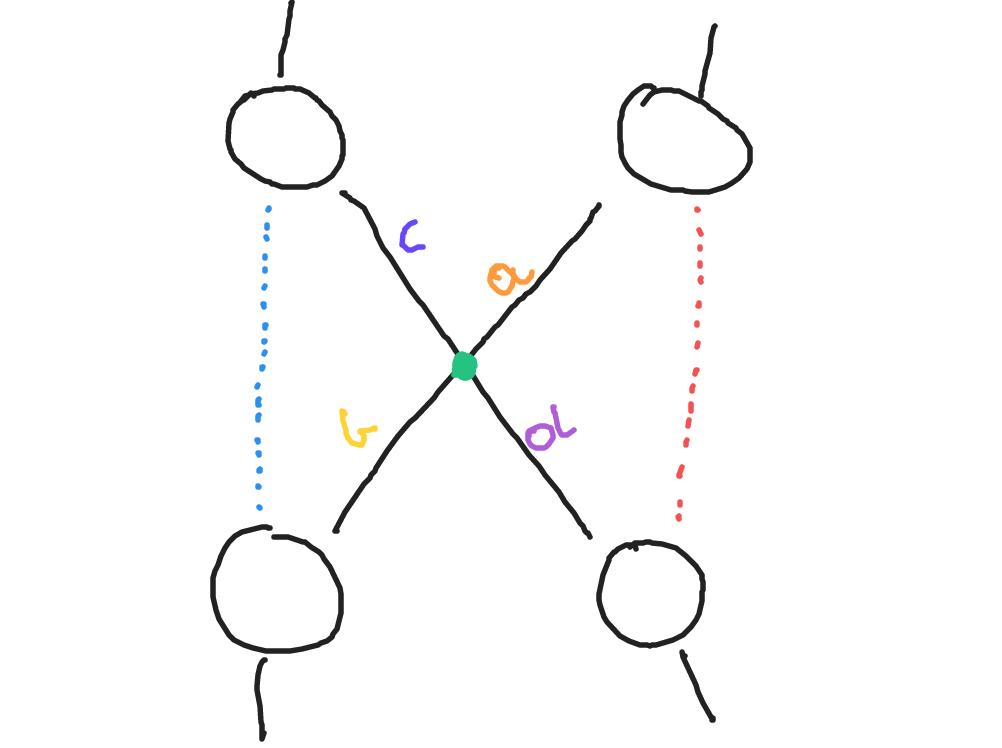
\includegraphics[scale=0.14]{5} 
\end{center}
As our cost function satisfies triangle inequality. Red direct edge won't have bigger weight than a + d, and Blue direct edge won't have bigger  weight then b + c. However, in circumstances where they are equal, all vertexes will be on one line.
\begin{center}
    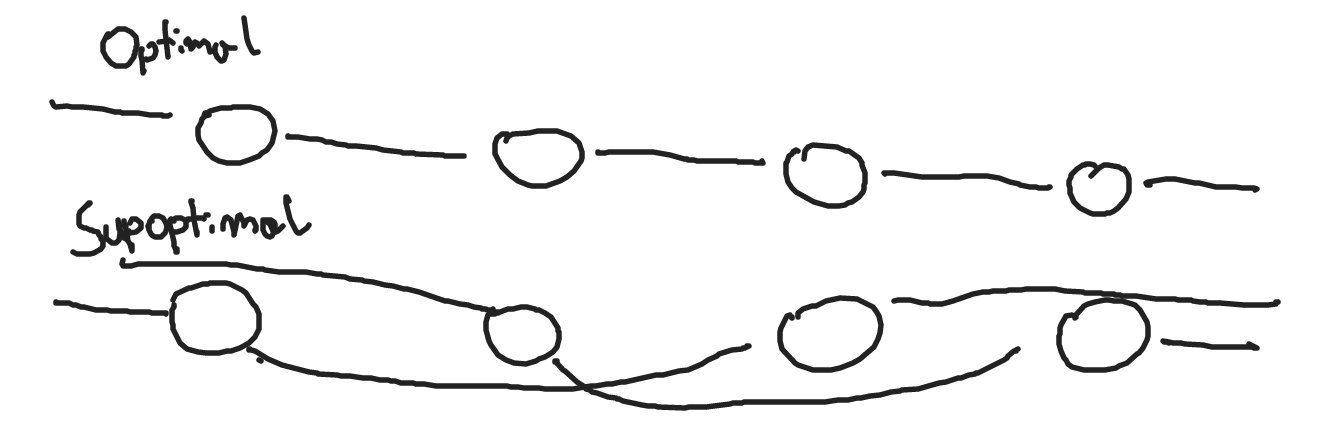
\includegraphics[scale=0.14]{6} 
\end{center}
Optimal solution in this case wouldn't have any crossing and should be created by taking cheapes edges. \\
\\
So in fact by splitting all crossings or taking cheapes edges in line circumstances we will create cycle that have smaller cost, contradiction.
\end{document}